\documentclass[12pt]{article}

\usepackage{amsmath}
\usepackage{amssymb}
\usepackage{amsthm}
\usepackage{geometry}
\usepackage{mathrsfs}
\usepackage{mathtools}
\usepackage{tikz}
\usetikzlibrary{arrows.meta, positioning, shapes, calc}
\usepackage{hyperref}

\geometry{letterpaper, margin=1in}

\title{Homework 2: Probability}
\author{Tashfeen Omran}
\date{September 2026}

\newtheorem{theorem}{Theorem}[section]
\newtheorem{lemma}[theorem]{Lemma}
\newtheorem{proposition}[theorem]{Proposition}
\newtheorem{corollary}[theorem]{Corollary}
\newtheorem{definition}{Definition}[section]
\newtheorem{axiom}{Axiom}[section]

\begin{document}

\maketitle
\tableofcontents
\newpage

\section{Part 1: Comprehensive Introduction, Context, and Prerequisites}

\subsection{Core Concepts \& Axioms}
Probability theory at its core is a rigorous branch of mathematics that formalizes randomness and uncertainty through measure theory and set theory. The foundational structure introduced in this chapter is the \textbf{Probability Space}, denoted typically by the triplet $(S, \mathcal{F}, P)$ in abstract math (where $S$ or $\Omega$ is the sample space). 

\begin{itemize}
    \item \textbf{Sample Space ($S$):} The set of all possible distinct outcomes of an experiment.
    \item \textbf{Event ($A$):} Any subset of the sample space $S$. In discrete cases, this is an element of the power set of $S$. 
    \item \textbf{Probability Measure ($P$):} A set-function that maps an event $A$ to a real number in the interval $[0,1]$, quantifying the likelihood of the event's occurrence.
\end{itemize}

The foundational bedrock of this discipline is provided by \textbf{Kolmogorov's Axioms} (Definition 2.6 in the text):
\begin{axiom}[Non-negativity]
For any event $A \subseteq S$, $P(A) \geq 0$.
\end{axiom}
\begin{axiom}[Normalization]
The probability of the entire sample space is unity: $P(S) = 1$.
\end{axiom}
\begin{axiom}[Countable Additivity]
If $A_1, A_2, A_3, \dots$ form a sequence of pairwise mutually exclusive events (i.e., $A_i \cap A_j = \emptyset$ for $i \neq j$), then:
\[ P(A_1 \cup A_2 \cup A_3 \cup \dots) = \sum_{i=1}^{\infty} P(A_i) \]
\end{axiom}

\subsection{Intuition and Set-Theoretic/Logical Foundations}
Every probabilistic statement is inherently a set-theoretic statement. When we say ``Event $A$ or Event $B$ occurs," we are evaluating the probability of their union, $P(A \cup B)$. When we speak of ``Event $A$ and Event $B$ occurring simultaneously," we are analyzing their intersection, $P(A \cap B)$. By partitioning the sample space $S$ into disjoint (mutually exclusive) sets, we can deconstruct highly complex real-world uncertainties into simple, summable scalar values. The logic here is spatial: think of probability as calculating the ``mass'' or ``area'' of a subset within a universal boundary $S$ that has a total mass of exactly $1$.

\subsection{Historical Context and Motivation}
Historically, probability began as an empirical heuristics tool for resolving gambling disputes, notably in the 1654 correspondence between Pierre de Fermat and Blaise Pascal. For centuries, probability relied on intuitive ``relative frequency'' limits or classical ``equally likely'' assumptions, which lacked mathematical rigor and led to profound foundational crises (e.g., Bertrand's Paradox). It was not until 1933 that Russian mathematician Andrey Kolmogorov axiomatized probability theory using the emerging tools of Lebesgue measure theory. This unified discrete and continuous probability into a single, rigorous mathematical framework that underpins modern quantitative science today.

\subsection{Key Theorems, Lemmas, and Formulas}
\begin{theorem}[Probability of a Complement]
For any event $A$, $P(\overline{A}) = 1 - P(A)$.
\end{theorem}
\begin{theorem}[Monotonicity of Probability]
If $A \subseteq B$, then $P(A) \leq P(B)$.
\end{theorem}
\begin{theorem}[General Addition Rule]
For any two events $A$ and $B$, $P(A \cup B) = P(A) + P(B) - P(A \cap B)$.
\end{theorem}
\begin{theorem}[Distributive Laws of Sets]
$A \cap (B \cup C) = (A \cap B) \cup (A \cap C)$ and $A \cup (B \cap C) = (A \cup B) \cap (A \cup C)$.
\end{theorem}
\begin{theorem}[De Morgan's Laws]
$\overline{(A \cup B)} = \overline{A} \cap \overline{B}$ and $\overline{(A \cap B)} = \overline{A} \cup \overline{B}$.
\end{theorem}

\subsection{Prerequisites}
To fully synthesize this material, mastery of the following is required:
\begin{itemize}
    \item \textbf{Naive Set Theory:} Operations including union, intersection, complement, and set difference.
    \item \textbf{Proof Techniques:} Direct proof, proof by contradiction, and algebraic manipulations of sets.
    \item \textbf{Combinatorics:} Basic counting principles, permutations, and combinations (e.g., $\binom{n}{k}$).
    \item \textbf{Real Analysis (Basic):} Understanding sequences, series convergence, and non-negative summations.
\end{itemize}

\newpage
\section{Part 2: Detailed Homework Solutions}

\textit{Note: As requested, the following is a strategic selection of problems from the homework assignment that rigorously represents every distinct problem archetype and problem-solving technique found in Chapter 2, including set operations, tabular empirical probability, the sample-point method, complex conditional logic, and axiomatic proofs.}

% ---------------- PROBLEM 2.5 ----------------
\subsection*{Exercise 2.5 (Set Identity Proofs)}
\textbf{Problem Statement:} Refer to Exercise 2.4. Use the identities $A = A \cap S$ and $S = B \cup \overline{B}$ and a distributive law to prove the following:
\begin{enumerate}
    \item[a.] $A = (A \cap B) \cup (A \cap \overline{B})$.
    \item[b.] If $B \subset A$ then $A = B \cup (A \cap \overline{B})$.
    \item[c.] Further, show that $(A \cap B)$ and $(A \cap \overline{B})$ are mutually exclusive and therefore that $A$ is the union of two mutually exclusive sets.
    \item[d.] Also show that $B$ and $(A \cap \overline{B})$ are mutually exclusive and if $B \subset A$, $A$ is the union of two mutually exclusive sets, $B$ and $(A \cap \overline{B})$.
\end{enumerate}

\begin{proof}[Solution to 2.5]
\textbf{Part (a):} Direct Proof using set definitions.
\begin{align*}
    A &= A \cap S \quad \text{(Intersection with the universal set yields the set itself)} \\
      &= A \cap (B \cup \overline{B}) \quad \text{(Since } S = B \cup \overline{B}\text{)} \\
      &= (A \cap B) \cup (A \cap \overline{B}) \quad \text{(By the Distributive Law of Intersection over Union)}.
\end{align*}
This proves the identity. 

\textbf{Part (b):} Direct Proof with Subset condition. \\
Assume $B \subset A$. By definition of a subset, every element in $B$ is also in $A$. Therefore, the intersection of $A$ and $B$ is simply $B$ itself. 
\[ A \cap B = B \]
Substituting this result into the identity proven in part (a):
\[ A = (A \cap B) \cup (A \cap \overline{B}) = B \cup (A \cap \overline{B}) \]

\textbf{Part (c):} Proof of mutual exclusivity. \\
Two sets are mutually exclusive if their intersection is the empty set ($\emptyset$). We evaluate the intersection of $(A \cap B)$ and $(A \cap \overline{B})$:
\begin{align*}
    (A \cap B) \cap (A \cap \overline{B}) &= A \cap (B \cap \overline{B}) \cap A \quad \text{(Associativity and Commutativity)} \\
    &= A \cap \emptyset \cap A \quad \text{(Since a set and its complement are disjoint, } B \cap \overline{B} = \emptyset\text{)} \\
    &= \emptyset \quad \text{(Intersection with the empty set is the empty set)}.
\end{align*}
Since their intersection is empty, $(A \cap B)$ and $(A \cap \overline{B})$ are mutually exclusive. From part (a), $A$ is constructed from their union.

\textbf{Part (d):} Proof of mutual exclusivity under subset conditions. \\
We check the intersection of $B$ and $(A \cap \overline{B})$:
\begin{align*}
    B \cap (A \cap \overline{B}) &= (B \cap \overline{B}) \cap A \quad \text{(Associativity and Commutativity)} \\
    &= \emptyset \cap A \\
    &= \emptyset.
\end{align*}
Thus, $B$ and $A \cap \overline{B}$ are mutually exclusive. From part (b), if $B \subset A$, then $A = B \cup (A \cap \overline{B})$. Consequently, $A$ is defined as the union of these two mutually exclusive sets. 
\end{proof}

% ---------------- PROBLEM 2.8 ----------------
\subsection*{Exercise 2.8 (Set Enumeration \& Sample Space)}
\textbf{Problem Statement:} Suppose two dice are tossed and the numbers on the upper faces are observed. Let $S$ denote the set of all possible pairs. 
a. Define the subsets of $S$:
$A$: The number on the second die is even.
$B$: The sum of the two numbers is even.
$C$: At least one number in the pair is odd.
b. List the points in $A, \overline{C}, A \cap B, A \cap \overline{B}, \overline{A} \cup B,$ and $\overline{A} \cap C$.

\begin{proof}[Solution to 2.8]
\textbf{Part (a): Setup of Probability Space} \\
Let the sample space be defined as $S = \{ (i,j) \mid i,j \in \{1,2,3,4,5,6\} \}$. The cardinality of $S$ is $|S| = 36$.
\begin{align*}
    A &= \{ (i,j) \in S \mid j \text{ is even} \} \\
    B &= \{ (i,j) \in S \mid (i+j) \text{ is even} \} \\
    C &= \{ (i,j) \in S \mid i \text{ is odd} \lor j \text{ is odd} \}
\end{align*}

\textbf{Part (b): Enumeration of Sample Points} \\
\noindent \textbf{Set $A$}: All pairs where the second die is 2, 4, or 6. 
\begin{align*}
A = \{ &(1,2), (2,2), (3,2), (4,2), (5,2), (6,2), \\
       &(1,4), (2,4), (3,4), (4,4), (5,4), (6,4), \\
       &(1,6), (2,6), (3,6), (4,6), (5,6), (6,6) \}
\end{align*}

\noindent \textbf{Set $\overline{C}$}: The complement of ``at least one odd'' is ``both are even''.
\begin{align*}
\overline{C} = \{ (2,2), (2,4), (2,6), (4,2), (4,4), (4,6), (6,2), (6,4), (6,6) \}
\end{align*}

\noindent \textbf{Set $A \cap B$}: The second die is even AND the sum is even. For the sum to be even while one addend is even, the other addend must also be even. Thus, this is the set where both dice are even, which is identically equal to $\overline{C}$.
\begin{align*}
A \cap B = \{ (2,2), (2,4), (2,6), (4,2), (4,4), (4,6), (6,2), (6,4), (6,6) \}
\end{align*}

\noindent \textbf{Set $A \cap \overline{B}$}: The second die is even AND the sum is odd. This forces the first die to be odd.
\begin{align*}
A \cap \overline{B} = \{ (1,2), (3,2), (5,2), (1,4), (3,4), (5,4), (1,6), (3,6), (5,6) \}
\end{align*}

\noindent \textbf{Set $\overline{A} \cup B$}: The second die is odd OR the sum is even. Note that if the sum is even ($B$), the dice are either (odd, odd) or (even, even). $\overline{A}$ contains all outcomes where the second die is odd. Thus, the union encompasses all instances where the second die is odd, plus all instances where both dice are even. 
\begin{align*}
\overline{A} \cup B = \{ &(1,1), (2,1), (3,1), (4,1), (5,1), (6,1), \\
                         &(1,3), (2,3), (3,3), (4,3), (5,3), (6,3), \\
                         &(1,5), (2,5), (3,5), (4,5), (5,5), (6,5), \\
                         &(2,2), (2,4), (2,6), (4,2), (4,4), (4,6), (6,2), (6,4), (6,6) \}
\end{align*}

\noindent \textbf{Set $\overline{A} \cap C$}: The second die is odd AND at least one is odd. Because the second die being odd strictly satisfies the condition of $C$, the intersection is simply $\overline{A}$ itself.
\begin{align*}
\overline{A} \cap C = \{ &(1,1), (2,1), (3,1), (4,1), (5,1), (6,1), \\
                         &(1,3), (2,3), (3,3), (4,3), (5,3), (6,3), \\
                         &(1,5), (2,5), (3,5), (4,5), (5,5), (6,5) \}
\end{align*}
\end{proof}

% ---------------- PROBLEM 2.14 ----------------
\subsection*{Exercise 2.14 (Empirical Probability Integration)}
\textbf{Problem Statement:} A survey classified adults by whether they need reading glasses and whether they use them. 
\begin{itemize}
    \item Needs: Yes | Uses: Yes (0.44), No (0.14)
    \item Needs: No | Uses: Yes (0.02), No (0.40)
\end{itemize}
Find the probabilities that the adult:
a. needs glasses. 
b. needs glasses but does not use them. 
c. uses glasses whether the glasses are needed or not.

\begin{proof}[Solution to 2.14]
Let the sample space consist of ordered pairs: $S = \{ (N, U) \}$ where $N \in \{Y, N\}$ denotes ``Needs glasses'' and $U \in \{Y, N\}$ denotes ``Uses glasses''. We are given the following mutually exclusive probability assignments:
\[ P(Y,Y) = 0.44, \quad P(Y,N) = 0.14, \quad P(N,Y) = 0.02, \quad P(N,N) = 0.40 \]

\textbf{Part (a):} Let $A$ be the event ``needs glasses''. This corresponds to all sample points where $N=Y$.
\[ A = \{ (Y,Y), (Y,N) \} \]
By Axiom 3 (addition over disjoint sets):
\[ P(A) = P(Y,Y) + P(Y,N) = 0.44 + 0.14 = 0.58 \]

\textbf{Part (b):} Let $B$ be the event ``needs glasses but does not use them''.
\[ B = \{ (Y,N) \} \]
\[ P(B) = P(Y,N) = 0.14 \]

\textbf{Part (c):} Let $C$ be the event ``uses glasses''. This corresponds to all sample points where $U=Y$.
\[ C = \{ (Y,Y), (N,Y) \} \]
By Axiom 3:
\[ P(C) = P(Y,Y) + P(N,Y) = 0.44 + 0.02 = 0.46 \]
\end{proof}

% ---------------- PROBLEM 2.20 ----------------
\subsection*{Exercise 2.20 (The Monty Hall Problem)}
\textbf{Problem Statement:} 
a. Assign reasonable probabilities to the simple events for a contestant selecting one of three curtains (one Good Prize $G$, two Duds $D_1, D_2$). 
b. Evaluate the logic of switching curtains after the host reveals a dud.
i. If she stays with her initial choice, what is the probability she wins?
ii. If she chooses $G$, host opens a dud, she switches. What is the result?
iii. If she chooses a dud, host opens the other dud, she switches. What is the result?
iv. What is the probability of winning if she switches?
v. Which strategy maximizes the probability of winning?

\begin{proof}[Solution to 2.20]
\textbf{Part (a):} Let $S$ denote the set of curtains the contestant can initially choose. 
\[ S = \{ G, D_1, D_2 \} \]
Assuming the contestant has no prior information, by the Principle of Indifference, each simple event is equally likely:
\[ P(G) = P(D_1) = P(D_2) = \frac{1}{3} \]
The probability of initially selecting the curtain with the nice prize is $P(G) = 1/3$.

\textbf{Part (b):} We map the game-theoretic outcomes of the contestant's actions:
\begin{enumerate}
    \item[i.] If the contestant strictly commits to \textit{staying}, she wins if and only if her initial random selection was $G$. The probability is exactly $P(G) = \frac{1}{3}$.
    \item[ii.] Suppose the contestant's initial choice is $G$. The host is forced to reveal one of the duds (say $D_1$). The remaining closed curtain is $D_2$. If the contestant \textit{switches}, she will switch from $G$ to $D_2$. \textbf{Result: She loses.}
    \item[iii.] Suppose the contestant's initial choice is one of the duds, say $D_1$. The host knows where the prize is and \textit{must} reveal a dud. Therefore, the host has no choice but to reveal $D_2$. The remaining closed curtain is $G$. If the contestant \textit{switches}, she will switch from $D_1$ to $G$. \textbf{Result: She wins.} (By symmetry, the exact same logic applies if she initially selected $D_2$).
    \item[iv.] Under a strict \textit{switching} strategy, the contestant wins if and only if her initial selection was a dud (as proven in ii and iii). Let $W_{\text{switch}}$ be the event of winning by switching. 
    \[ W_{\text{switch}} = \{ D_1, D_2 \} \]
    By Axiom 3, $P(W_{\text{switch}}) = P(D_1) + P(D_2) = \frac{1}{3} + \frac{1}{3} = \frac{2}{3}$.
    \item[v.] The probability of winning by switching ($\frac{2}{3}$) is strictly greater than the probability of winning by staying ($\frac{1}{3}$). Therefore, \textbf{switching} is the strategy that maximizes the probability of winning the Good Prize.
\end{enumerate}
\end{proof}

% ---------------- PROBLEM 2.21 ----------------
\subsection*{Exercise 2.21 (Axiomatic Proof of the Total Probability Law)}
\textbf{Problem Statement:} If $A$ and $B$ are events, use the result derived in Exercise 2.5(a) and the Axioms in Definition 2.6 to prove that $P(A) = P(A \cap B) + P(A \cap \overline{B})$.

\begin{proof}[Solution to 2.21]
We are given an arbitrary probability space containing events $A$ and $B$.
\begin{enumerate}
    \item From Exercise 2.5(a), we established the set equivalence:
    \[ A = (A \cap B) \cup (A \cap \overline{B}) \]
    \item From Exercise 2.5(c), we rigorously proved that the sets $(A \cap B)$ and $(A \cap \overline{B})$ are mutually exclusive, meaning their intersection is the empty set $\emptyset$.
    \item Axiom 3 (Countable Additivity) states that the probability of the union of mutually exclusive events is equal to the sum of their individual probabilities.
    \item Applying Axiom 3 to the union derived in step 1 yields:
    \[ P(A) = P\Big( (A \cap B) \cup (A \cap \overline{B}) \Big) = P(A \cap B) + P(A \cap \overline{B}) \]
\end{enumerate}
This completes the proof.
\end{proof}

% ---------------- PROBLEM 2.24 ----------------
\subsection*{Exercise 2.24 (Axiomatic Proof of Monotonicity)}
\textbf{Problem Statement:} Use the result in Exercise 2.22 (which states if $A \subset B$, $P(B) = P(A) + P(B \cap \overline{A})$) and the Axioms to prove that if $A \subset B$, then $P(A) \leq P(B)$.

\begin{proof}[Solution to 2.24]
Let $A$ and $B$ be events such that $A \subset B$.
\begin{enumerate}
    \item From the referenced exercise, we possess the established equality:
    \[ P(B) = P(A) + P(B \cap \overline{A}) \]
    \item By Axiom 1 (Non-negativity), the probability of any event in the sample space must be greater than or equal to zero. Therefore, applying this axiom to the event $(B \cap \overline{A})$:
    \[ P(B \cap \overline{A}) \geq 0 \]
    \item We can manipulate the equality from step 1 algebraically:
    \[ P(B) - P(A) = P(B \cap \overline{A}) \]
    \item Substituting the inequality from step 2 into step 3:
    \[ P(B) - P(A) \geq 0 \]
    \item Adding $P(A)$ to both sides of the inequality yields the final result:
    \[ P(B) \geq P(A) \quad \text{or} \quad P(A) \leq P(B) \]
\end{enumerate}
This confirms that probability measures are monotonically non-decreasing with respect to set inclusion.
\end{proof}

% ---------------- PROBLEM 2.29 ----------------
\subsection*{Exercise 2.29 (Combinatorics and Sample Points)}
\textbf{Problem Statement:} Two additional jurors are needed to complete a jury. There are six prospective jurors: two women and four men. Two jurors are randomly selected. 
a. Define the experiment and one sample point.
b. List the sample space associated with this experiment.
c. What is the probability that both of the jurors selected are women?

\begin{proof}[Solution to 2.29]
\textbf{Part (a):} The experiment consists of randomly selecting an unordered pair of individuals from a finite population of six distinct individuals without replacement. A single sample point represents one specific pair of chosen jurors.

\textbf{Part (b):} Let the women be denoted as $W_1$ and $W_2$. Let the men be denoted as $M_1, M_2, M_3, M_4$. The sample space $S$ consists of all subsets of size exactly two. The total number of sample points is given by the combination $\binom{6}{2} = \frac{6!}{2!4!} = 15$.
The sample space is fully enumerated as:
\begin{align*}
S = \big\{ &\{W_1, W_2\}, \{W_1, M_1\}, \{W_1, M_2\}, \{W_1, M_3\}, \{W_1, M_4\}, \\
           &\{W_2, M_1\}, \{W_2, M_2\}, \{W_2, M_3\}, \{W_2, M_4\}, \\
           &\{M_1, M_2\}, \{M_1, M_3\}, \{M_1, M_4\}, \\
           &\{M_2, M_3\}, \{M_2, M_4\}, \\
           &\{M_3, M_4\} \big\}
\end{align*}

\textbf{Part (c):} Let $E$ be the event that ``both jurors selected are women''. By examining our enumerated sample space $S$, we see that exactly one sample point satisfies this criteria:
\[ E = \{ \{W_1, W_2\} \} \]
Because the jurors are selected entirely at random, each of the 15 distinct sample points is an equally likely outcome. Therefore, the probability of selecting any specific sample point is $\frac{1}{15}$.
\[ P(E) = \frac{|E|}{|S|} = \frac{1}{15} \]
\end{proof}

\newpage
\section{Part 3: In-Depth Analysis of Problems and Techniques}

\subsection{A) Problem Types and Logical Strategies}
The problems in this foundational chapter can be meticulously categorized into three predominant archetypes:
\begin{itemize}
    \item \textbf{Set-Theoretic Algebraic Proofs (Problems 2.5, 2.21, 2.24):} These require translating probability questions entirely into set theory. The overarching strategy is absolute reliance on De Morgan's Laws and Distributive Laws to rewrite complex set operations into unions of mutually exclusive subsets. Once mutual exclusivity is established algebraically ($A \cap B = \emptyset$), one bridges the gap to probability via Axiom 3.
    \item \textbf{Sample-Point Combinatorics (Problems 2.8, 2.29):} Here, the probability space is finite and discrete. The strategy is exhaustive enumeration or combinatorial calculation ($\binom{n}{k}$) to define the size of the total sample space $S$. Probabilities are computed via ratio $|A|/|S|$ under the assumption of equiprobability (the discrete uniform measure).
    \item \textbf{Conditional Information and Game Logic (Problem 2.20):} The Monty Hall problem represents an advanced class of probabilistic modeling where the sample space shifts conditionally based on an agent's actions. The strategy is to explicitly map the entire chronological decision tree, assign probabilities to the root nodes, and follow the deterministic deterministic paths to verify the true probabilities of final outcomes.
\end{itemize}

\subsection{B) Key Analytical and Logical Manipulations}
\begin{itemize}
    \item \textbf{The Partition Trick (Law of Total Probability Base):} In Exercise 2.21, rewriting $A$ as $(A \cap B) \cup (A \cap \overline{B})$ was not merely an algebra trick; it is the fundamental mechanism behind the Law of Total Probability. It allows us to calculate the probability of a complex event $A$ by conditioning it on a simpler, binary event partition ($B$ and $\overline{B}$).
    \item \textbf{Complement Subtraction:} Identifying that $A \cap (B \cap \overline{B}) = \emptyset$ (Problem 2.5c) leverages the Law of Non-Contradiction from formal logic (a statement cannot be both true and false). This manipulation is vital when verifying that our partitioned spaces do not ``double count'' probabilities.
    \item \textbf{Translation of Inequality:} In Problem 2.24, the mathematical technique of proving an inequality $P(A) \leq P(B)$ relied on proving that their difference equals a non-negative quantity. This is a universally powerful technique in real analysis and measure theory. 
\end{itemize}

\newpage
\section{Part 4: Cheatsheet, Visuals, and Tips for Success}

\subsection{Theoretical Visual: Partitioning the Probability Measure}
The following TikZ visual illustrates the fundamental trick used in Exercise 2.5 and 2.21: partitioning a Sample Space $\Omega$ (denoted $S$ in the text) and an event $A$ using an intersecting set $B$. This visual confirms that $A = (A \cap B) \cup (A \cap \overline{B})$.

\vspace{0.5cm}
\begin{center}
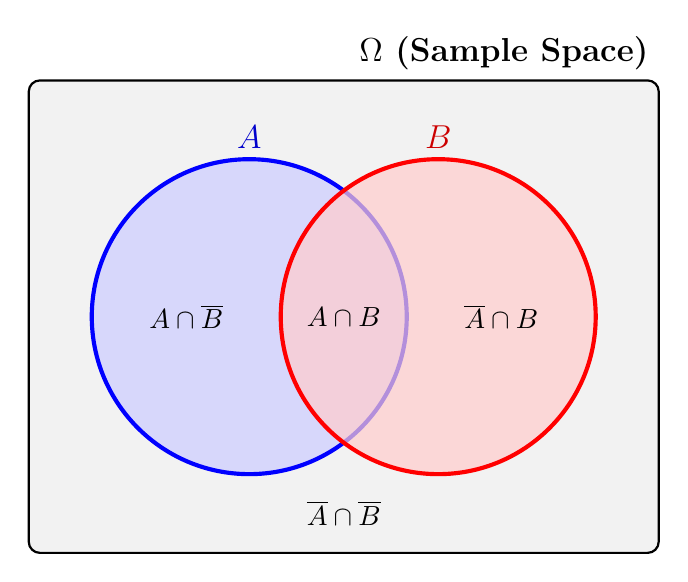
\begin{tikzpicture}[thick]
  % Define the universe (Sample Space)
  \draw[rounded corners, fill=gray!10] (-4, -3) rectangle (4, 3);
  \node[anchor=south east, font=\large\bfseries] at (4, 3) {$\Omega$ (Sample Space)};

  % Define set A
  \begin{scope}[shift={(-1.2,0)}]
    \draw[fill=blue!20, fill opacity=0.7, draw=blue, line width=1.5pt] (0,0) circle (2cm);
    \node[blue!80!black, font=\large\bfseries, anchor=south] at (0, 2) {$A$};
  \end{scope}

  % Define set B
  \begin{scope}[shift={(1.2,0)}]
    \draw[fill=red!20, fill opacity=0.7, draw=red, line width=1.5pt] (0,0) circle (2cm);
    \node[red!80!black, font=\large\bfseries, anchor=south] at (0, 2) {$B$};
  \end{scope}

  % Labels for partitions
  \node[font=\bfseries] at (-2, 0) {$A \cap \overline{B}$};
  \node[font=\bfseries] at (0, 0) {$A \cap B$};
  \node[font=\bfseries] at (2, 0) {$\overline{A} \cap B$};
  \node[font=\bfseries] at (0, -2.5) {$\overline{A} \cap \overline{B}$};
\end{tikzpicture}
\end{center}
\vspace{0.5cm}

\subsection{Heuristics \& ``Cheats''}
\begin{itemize}
    \item \textbf{The ``At Least One'' Shortcut:} Whenever a problem asks for the probability of ``at least one'' entity possessing a trait (e.g., Problem 2.8c), immediately calculate $1 - P(\text{None})$. This avoids summing combinations. 
    \item \textbf{Indicator Functions:} While not explicitly required yet, mentally assigning $1$ if an outcome is in a set and $0$ if it is not transforms set logic into basic binary arithmetic (Boolean Algebra). 
\end{itemize}

\subsection{Pitfalls \& Fallacies}
\begin{itemize}
    \item \textbf{The Independence vs. Mutually Exclusive Fallacy:} The most dangerous trap in introductory probability. Mutually exclusive events (that have non-zero probability) are \textbf{never} independent. If they are mutually exclusive, $P(A \cap B) = 0$. If they were independent, $P(A \cap B) = P(A)P(B) > 0$. Do not confuse the two properties.
    \item \textbf{The Union Bound Trap:} Assuming $P(A \cup B) = P(A) + P(B)$ without first rigorously proving that $A \cap B = \emptyset$. Always default to the General Addition Rule.
\end{itemize}

\newpage
\section{Part 5: Conceptual Synthesis and The ``Big Picture''}

\subsection{A) Thematic Connections}
The central unifying theme of this topic is the \textbf{translation of qualitative uncertainty into strict quantitative measure spaces}. By applying rigorous set theory, we construct a mathematically impermeable bridge between philosophical concepts of ``chance'' and pure algebra. This theme unifies prior mathematical topics: the integration of combinatorics (for counting sample points), Boolean logic (for set intersections and unions), and basic geometry (measuring the abstract ``area'' of overlapping shapes).

\subsection{B) Forward and Backward Links}
\begin{itemize}
    \item \textbf{Backward Link:} The axioms of probability are mathematically identical to the axioms defining mass and length in classical physics. You are applying the geometric logic you already know to abstract outcome spaces. 
    \item \textbf{Forward Link:} The foundational definitions of $\sigma$-algebras and subsets built here are absolute prerequisites for Random Variables (functions mapping from $S$ to $\mathbb{R}$) and Lebesgue Integration. In advanced Stochastic Calculus, these exact partitioned sets will evolve into ``Filtrations'' ($\mathcal{F}_t$), which track the mathematical flow of information over time to prove whether a trading strategy contains arbitrage. 
\end{itemize}

\section{Part 6: Abstract Real-World Modeling (AI, ML, \& Quant Finance)}

\subsection{A) Concrete Scenarios}
\begin{itemize}
    \item \textbf{Machine Learning (Bayesian Classifier Spaces):} In Natural Language Processing, a generative AI model calculates the probability of a word given prior context. The model relies on a vast discrete sample space partitioned by conditional constraints (just like our derivations in Exercise 2.21, utilizing the Total Probability rule recursively over billions of parameter intersections).
    \item \textbf{Quantitative Finance (Measure Theory and Derivative Pricing):} In modern Quant trading, the Black-Scholes framework relies on calculating probabilities of asset price movements. However, market prices contain risk premia. Quants must utilize Girsanov's Theorem to mathematically shift from the ``real-world'' physical probability measure $\mathbb{P}$ to a ``risk-neutral'' measure $\mathbb{Q}$. This mathematical shift is only valid if both measures agree on which events have a probability of $0$ (equivalent probability spaces).
\end{itemize}

\subsection{B) Model Problem Setup: The Discrete Equivalent Martingale Model}
To model a financial derivative rigorously using the probability concepts mastered in this chapter, we define a one-period stochastic asset pricing model. 
\vspace{0.2cm}\\
\noindent \textbf{State Space & Random Variables:} \\
Let the sample space of market outcomes be $\Omega = \{ \omega_{\text{up}}, \omega_{\text{down}} \}$. Let $\mathcal{F}$ be the power set of $\Omega$. We define a real-world probability measure $\mathbb{P}$ such that $\mathbb{P}(\{\omega_{\text{up}}\}) = p$ and $\mathbb{P}(\{\omega_{\text{down}}\}) = 1-p$. 
We define a Random Variable $S_1$ (stock price at time 1) acting on $\Omega$:
\[ S_1(\omega_{\text{up}}) = S_0 u, \quad S_1(\omega_{\text{down}}) = S_0 d \]
where $S_0$ is the current stock price, and $u > 1 + r > d$ (where $r$ is the risk-free rate).

\noindent \textbf{Theoretical Optimization (Finding the Risk-Neutral Measure):} \\
By the Fundamental Theorem of Asset Pricing, to eliminate arbitrage, there must exist an equivalent probability measure $\mathbb{Q}$ such that the discounted expected value of the asset equals its current price. We define $\mathbb{Q}(\{\omega_{\text{up}}\}) = q$. We solve the linear constraint:
\[ S_0 = \frac{1}{1+r} \Big( q S_1(\omega_{\text{up}}) + (1-q) S_1(\omega_{\text{down}}) \Big) \]
\[ S_0 (1+r) = q(S_0 u) + (1-q)(S_0 d) \]
\[ 1+r = qu + d - qd \implies q = \frac{(1+r) - d}{u - d} \]
Because $u > 1+r > d$, we are guaranteed that $0 < q < 1$. Thus, $\mathbb{Q}$ perfectly satisfies Kolmogorov's Axioms established in this chapter, granting us a mathematically robust mechanism to price complex derivative securities without assuming real-world directional risk!

\newpage
\section{Part 7: Common Variations and Untested Concepts}

The provided homework assignments meticulously cover two-event scenarios and discrete finite enumerations. However, advanced probability exams frequently test generalizations of these concepts that are critically missing from this specific assignment set.

\subsection{Missing Concept 1: The Principle of Inclusion-Exclusion (3+ Events)}
The homework required proving $P(A \cup B) = P(A) + P(B) - P(A \cap B)$. A common exam variation extends this to three events.
\begin{theorem}
For any events $A, B,$ and $C$:
\begin{align*}
P(A \cup B \cup C) &= P(A) + P(B) + P(C) \\
&\quad - P(A \cap B) - P(A \cap C) - P(B \cap C) \\
&\quad + P(A \cap B \cap C)
\end{align*}
\end{theorem}
\begin{proof}
Treat $(B \cup C)$ as a single composite event $D$. By the two-event rule:
\[ P(A \cup D) = P(A) + P(D) - P(A \cap D) \]
Substitute $D = B \cup C$: 
\[ P(D) = P(B) + P(C) - P(B \cap C) \]
For the intersection term, apply the Distributive Law:
\[ P(A \cap D) = P\Big( A \cap (B \cup C) \Big) = P\Big( (A \cap B) \cup (A \cap C) \Big) \]
Applying the two-event rule to this union yields:
\[ P(A \cap D) = P(A \cap B) + P(A \cap C) - P\Big( (A \cap B) \cap (A \cap C) \Big) \]
Since $(A \cap B) \cap (A \cap C) = A \cap B \cap C$, substituting all expansions back into the original equation yields the theorem perfectly.
\end{proof}

\subsection{Missing Concept 2: Continuity of Probability Measures}
Advanced courses bridge discrete sample spaces to continuous spaces (calculus) by treating probability measures as continuous functions on nested sets. 
\begin{theorem}
Let $\{A_n\}$ be an increasing sequence of events such that $A_1 \subseteq A_2 \subseteq A_3 \subseteq \dots$ and let $A = \bigcup_{n=1}^\infty A_n$. Then, $P(A) = \lim_{n \to \infty} P(A_n)$.
\end{theorem}
\begin{proof}
We construct a sequence of \textit{mutually exclusive} sets to apply Axiom 3. Let $B_1 = A_1$, and for $n \geq 2$, $B_n = A_n \cap \overline{A_{n-1}}$. The disjoint union $\bigcup_{i=1}^\infty B_i = A$.
By Axiom 3:
\[ P(A) = P\Big( \bigcup_{i=1}^\infty B_i \Big) = \sum_{i=1}^\infty P(B_i) = \lim_{n \to \infty} \sum_{i=1}^n P(B_i) \]
Note that $\bigcup_{i=1}^n B_i$ is identically equal to $A_n$. Therefore, the finite sum $\sum_{i=1}^n P(B_i) = P(A_n)$. Thus:
\[ P(A) = \lim_{n \to \infty} P(A_n) \]
This confirms probability behaves identically to limits in Real Analysis.
\end{proof}

\newpage
\section{Part 8: Advanced Diagnostic Testing: ``Find the Flaw''}
\textit{Task: Act as the grader. Identify the specific subtle logical, mathematical, or set-theoretic error in each proof below. Justify your correction. (Solutions are on the final page).}

\subsection*{Problem 1: The Union Subadditivity ``Proof''}
\textbf{Conjecture:} For any two events $A$ and $B$, $P(A \cup B) = P(A) + P(B)$. \\
\textbf{Proof Given:} Let $A$ and $B$ be subsets of a valid probability space $S$. The set operation $A \cup B$ groups together all sample points in $A$ and all sample points in $B$. By Kolmogorov's third axiom of probability, the probability of a combined grouping is equal to the sum of the probabilities of its composite sets. Therefore, $P(A \cup B) = P(A) + P(B)$. $\blacksquare$

\subsection*{Problem 2: The Subset Reversal Re-Arrangement}
\textbf{Conjecture:} If event $A$ is a subset of event $B$ ($A \subset B$), then $P(A) \geq P(B)$. \\
\textbf{Proof Given:} Since $A \subset B$, we can write $B$ as the union of $A$ and the part of $B$ not in $A$. That is, $B = A \cup (B \cap \overline{A})$. Because $A$ and $(B \cap \overline{A})$ are disjoint, Axiom 3 dictates $P(B) = P(A) + P(B \cap \overline{A})$. Since probability values must be non-negative (Axiom 1), adding $P(B \cap \overline{A})$ to $P(A)$ will only increase the total. This mathematically ensures that $P(A) \geq P(B)$. $\blacksquare$

\subsection*{Problem 3: The Infinite Uniform Sample Space Paradox}
\textbf{Conjecture:} A uniform probability distribution cannot exist over a countably infinite sample space. \\
\textbf{Proof Given:} Let $S = \{1, 2, 3, \dots \}$ be an infinite sample space. Assume a uniform probability measure exists, such that $P(\{i\}) = c > 0$ for all integers $i$. By Axiom 2 and 3, $1 = P(S) = \sum_{i=1}^\infty P(\{i\}) = \sum_{i=1}^\infty c$. Because adding a strictly positive constant infinite times yields infinity, $1 = \infty$, a mathematical contradiction. Thus, $c$ must equal $0$. Since $c=0$, $P(S) = \sum 0 = 0$, violating Axiom 2. Therefore, no probability measure can exist on an infinite sample space. $\blacksquare$

\subsection*{Problem 4: The Void of Probability Zero}
\textbf{Conjecture:} If an event has a probability of exactly zero, it is impossible for the event to occur. \\
\textbf{Proof Given:} By Axiom 1, $P(A) \geq 0$ for all events. We know that the probability of the empty set $P(\emptyset) = 0$. Since the empty set contains zero sample points, it mathematically represents an impossible outcome. Therefore, if we are given an event $X$ such that $P(X) = 0$, by algebraic substitution, $X$ must equal $\emptyset$. Thus, event $X$ is entirely impossible. $\blacksquare$

\subsection*{Problem 5: The Independence Equivalence}
\textbf{Conjecture:} If events $A$ and $B$ are mutually exclusive, and neither is the empty set, they must be independent events. \\
\textbf{Proof Given:} Let $A$ and $B$ be mutually exclusive subsets. This implies that they occupy completely distinct, non-overlapping geometric locations in the sample space $S$. Because they do not overlap, the occurrence of event $A$ mathematically does not touch or affect event $B$. Since their occurrence does not affect one another, they are independent. $\blacksquare$

\newpage
\subsection*{Solution Key to Diagnostic Testing}

\textbf{Resolution to Problem 1 (The Disjoint Fallacy):}
\begin{itemize}
    \item \textbf{The Flaw:} The proof illicitly invokes Axiom 3 (Countable Additivity) without verifying its prerequisite constraint. Axiom 3 \textit{only} applies when the sets in the union are pairwise mutually exclusive (disjoint). 
    \item \textbf{The Correction:} If $A$ and $B$ intersect ($A \cap B \neq \emptyset$), the summation double-counts their overlap. The correct mathematical formula must subtract the intersection: $P(A \cup B) = P(A) + P(B) - P(A \cap B)$.
\end{itemize}

\textbf{Resolution to Problem 2 (Algebraic Subadditivity Reversal):}
\begin{itemize}
    \item \textbf{The Flaw:} The flaw lies in the final algebraic deduction. The student writes $P(B) = P(A) + (\text{a non-negative number})$. The student incorrectly concludes this means $P(A) \geq P(B)$.
    \item \textbf{The Correction:} If you take a number $P(A)$ and add a positive quantity to it to reach $P(B)$, then $P(A)$ must be \textit{smaller} than $P(B)$. Rearranging the correct equation yields $P(B) - P(B \cap \overline{A}) = P(A)$. Because $P(B \cap \overline{A}) \geq 0$, it follows strictly that $P(A) \leq P(B)$.
\end{itemize}

\textbf{Resolution to Problem 3 (Conflating Uniformity with all Measures):}
\begin{itemize}
    \item \textbf{The Flaw:} The student successfully proves that a \textit{uniform} distribution (where every outcome has the exact same non-zero probability $c$) is impossible over a countably infinite sample space. However, they falsely conclude that \textit{no} probability measure can exist.
    \item \textbf{The Correction:} We can easily assign non-uniform probabilities that converge. For example, assigning $P(\{i\}) = (\frac{1}{2})^i$ yields an infinite sum $\sum_{i=1}^\infty (\frac{1}{2})^i = 1$, perfectly satisfying Axioms 2 and 3.
\end{itemize}

\textbf{Resolution to Problem 4 (The Empty Set Confusion):}
\begin{itemize}
    \item \textbf{The Flaw:} The logical structure relies on the fallacy of Affirming the Consequent. The proof assumes that because $P(\emptyset) = 0$, then $P(X) = 0 \implies X = \emptyset$. This is a bi-directional assumption that is fundamentally false in calculus-based probability.
    \item \textbf{The Correction:} In continuous probability distributions (e.g., measuring the exact height of a human to infinite decimal places), the probability of observing any single, specific point is exactly $0$. However, that specific point exists in the sample space and is functionally possible! Thus, $P(X) = 0$ does not strictly mandate $X = \emptyset$.
\end{itemize}

\textbf{Resolution to Problem 5 (The Independence Traps):}
\begin{itemize}
    \item \textbf{The Flaw:} The student conflates physical/geometric non-intersection with probabilistic independence. This is the most famous pitfall in applied probability. 
    \item \textbf{The Correction:} If two events are mutually exclusive (and have positive probabilities), they are actually completely, heavily dependent! If event $A$ occurs, because they cannot overlap, you know with $100\%$ mathematical certainty that event $B$ did \textbf{not} occur. By definition, independence dictates that $P(A \cap B) = P(A)P(B) > 0$. But since they are mutually exclusive, $P(A \cap B) = 0$. Thus, $0 \neq P(A)P(B)$, proving they are definitively not independent. 
\end{itemize}

\end{document}